\section{Experiment}
\label{sec:exp}
\noindent\textbf{Datasets and metrics.}
We utilize two synthetic datasets, Shiny Blender~\cite{verbin2022refnerf} and Glossy Synthetic~\cite{liu2023nero}, along with the real-world Shiny Real dataset~\cite{verbin2022refnerf} to evaluating novel view synthesis of reflective objects. For quantitative assessment, we employ three standard image quality metrics: PSNR, SSIM~\cite{ssim}, and LPIPS ~\cite{lpips}, complemented by Mean Angular Error (MAE) for normal estimation accuracy.

\begin{table}[]
\centering
\captionsetup{width=0.99\linewidth}
\caption{Quantitative comparison on normal maps}
\label{tab:normal_compa}
\resizebox{0.99\columnwidth}{!}{%
\begin{tabular}{l|cccc}
\hline
\hline
Metrics & \multicolumn{4}{c}{Model}                                  \\ \hline
        & GShader\cite{jiang2024gaussianshader} & 3DGS-DR\cite{ye20243dgsdr} & Ref-Gaussian\cite{yao2024refgaussian} & Ours                          \\ \hline
MAE ↓   & 4.74    & 9.49    & 2.28   & \cellcolor[HTML]{FD6864}2.16  \\
SSIM ↑  & 0.853   & 0.824   & 0.924  & \cellcolor[HTML]{FD6864}0.924 \\
LPIPS ↓ & 0.108   & 0.172   & 0.073  & \cellcolor[HTML]{FD6864}0.072 \\ \hline
\hline
\end{tabular}%
}
\vspace{-1em}
\end{table}

% Please add the following required packages to your document preamble:
% \usepackage{graphicx}
% \usepackage[table,xcdraw]{xcolor}
% Beamer presentation requires \usepackage{colortbl} instead of \usepackage[table,xcdraw]{xcolor}
\begin{table*}[h!]
\vspace{-1em}
\centering
\captionsetup{width=0.9\textwidth}
\caption{Quantitative comparisons of relighting results in terms of PSNR↑ on the Glossy Synthetic dataset~\cite{liu2023nero}.}
\label{tab:relight_psnr}
\renewcommand{\arraystretch}{0.9}
\footnotesize
\resizebox{0.85\textwidth}{!}{%
\begin{tabular}{lccccccccc}
\hline
\hline
\multicolumn{1}{l|}{\textbf{Datasets}} & \textbf{angel} & \textbf{bell} & \textbf{cat} & \textbf{horse} & \textbf{luyu} & \textbf{potion} & \textbf{tbell} & \textbf{teapot} & \textbf{avg.} \\ \hline
\multicolumn{10}{c}{\textbf{corridor}} \\ \hline
\multicolumn{1}{l|}{GShader\cite{jiang2024gaussianshader}} & 21.83 & 22.98 & 16.42 & \cellcolor[HTML]{FD6864}26.42 & 16.74 & 14.99 & 18.74 & 20.35 & 19.81 \\
\multicolumn{1}{l|}{Ref-Gaussian\cite{yao2024refgaussian}} & 20.97 & 23.02 & 20.57 & 25.45 & 20.34 & 20.22 & 21.51 & 22.59 & 21.83 \\
\multicolumn{1}{l|}{IRGS\cite{gu2025irgs}} & 20.31 & 21.16 & 22.40 & 22.25 & 24.65 & 24.53 & 20.71 & 20.05 & 22.01 \\
\multicolumn{1}{l|}{Ours} & \cellcolor[HTML]{FD6864}23.92 & \cellcolor[HTML]{FD6864}25.76 & \cellcolor[HTML]{FD6864}27.32 & 25.80 & \cellcolor[HTML]{FD6864}25.11 & \cellcolor[HTML]{FD6864}27.42 & \cellcolor[HTML]{FD6864}24.61 & \cellcolor[HTML]{FD6864}26.05 & \cellcolor[HTML]{FD6864}25.75 \\ \hline
\multicolumn{10}{c}{\textbf{golf}} \\ \hline
\multicolumn{1}{l|}{GShader\cite{jiang2024gaussianshader}} & 21.04 & 21.40 & 14.84 & 25.01 & 14.85 & 12.65 & 16.80 & 18.50 & 18.14 \\
\multicolumn{1}{l|}{Ref-Gaussian\cite{yao2024refgaussian}} & 22.32 & 23.05 & 21.57 & 25.87 & 19.41 & 19.85 & 19.96 & 21.54 & 21.69 \\
\multicolumn{1}{l|}{IRGS\cite{gu2025irgs}} & 20.58 & 20.89 & 21.96 & 22.24 & 22.64 & 22.52 & 18.90 & 18.56 & 21.04 \\
\multicolumn{1}{l|}{Ours} & \cellcolor[HTML]{FD6864}26.37 & \cellcolor[HTML]{FD6864}26.99 & \cellcolor[HTML]{FD6864}27.35 & \cellcolor[HTML]{FD6864}26.28 & \cellcolor[HTML]{FD6864}24.85 & \cellcolor[HTML]{FD6864}26.14 & \cellcolor[HTML]{FD6864}23.91 & \cellcolor[HTML]{FD6864}26.19 & \cellcolor[HTML]{FD6864}26.01 \\ \hline
\multicolumn{10}{c}{\textbf{neon}} \\ \hline
\multicolumn{1}{l|}{GShader\cite{jiang2024gaussianshader}} & 21.16 & 21.41 & 16.74 & 24.12 & 16.87 & 15.59 & 18.94 & 19.07 & 19.24 \\
\multicolumn{1}{l|}{Ref-Gaussian\cite{yao2024refgaussian}} & 21.20 & \cellcolor[HTML]{FD6864}21.85 & 20.56 & 23.32 & 20.41 & 20.23 & 21.65 & 21.64 & 21.36 \\
\multicolumn{1}{l|}{IRGS\cite{gu2025irgs}} & 20.30 & 19.75 & 21.33 & 21.29 & 20.27 & 20.69 & 18.71 & 18.64 & 20.12 \\
\multicolumn{1}{l|}{Ours} & \cellcolor[HTML]{FD6864}21.72 & 21.36 & \cellcolor[HTML]{FD6864}25.31 & \cellcolor[HTML]{FD6864}24.52 & \cellcolor[HTML]{FD6864}21.65 & \cellcolor[HTML]{FD6864}23.66 & \cellcolor[HTML]{FD6864}21.87 & \cellcolor[HTML]{FD6864}22.93 & \cellcolor[HTML]{FD6864}22.88 \\ \hline
\hline
\end{tabular}%
}
\vspace{-1em}
\end{table*}

\noindent\textbf{Implementation details.}
All experiments run on a single NVIDIA RTX 3090 GPU. Our training pipeline follows the two-stage process in Sec~\ref{sec:method}. The first stage trains for 50,000 iterations with hyperparameters: $\lambda_{\mathrm{n}} = 0.05$, $\lambda_{\mathrm{d}} = 0.05$, $\lambda_{\text{smooth}} = 0.01$, $\lambda_{\text{geo-n}} = 0.005$, and $\lambda_{\text{geo-d}} = 0.005$. We use Marigold fine-tuned for normal and depth estimation due to its superior object-level prediction. The environmental lighting employs a $6 \times 128 \times 128$ mipmap cubemap with 3 RGB channels. The second stage performs 20,000 iterations of inverse rendering with $\lambda_{\text{smooth}} = 2.0$ and $\lambda_{\text{light}} = 0.01$. The learning rates are set to 0.0075 for albedo, 0.005 for roughness, 0.005 for metallic, and 0.01 for cubemap. Ray tracing uses IRGS~\cite{gu2025irgs} hyperparameters while other settings follow 2DGS~\cite{huang20242dgs}. The output at this stage enables direct relighting with ray samples increased to 2048 for improved quality. For enhanced novel view synthesis, we perform up to 80,000 specular compensation iterations with geometry, materials and lighting frozen. Only the spherical encoding components are updated, including an $8 \times 512 \times 512$ mipmap with 16 feature channels and a shallow MLP that has two 256-unit hidden layers. The total training without specular compensation takes approximately 80 minutes: 40 minutes for Stage I~\ref{sec:method-geo} and 40 minutes for Stage II~\ref{sec:method-ir}. Specular compensation requires an additional hour.

\begin{figure}[]
    \centering
    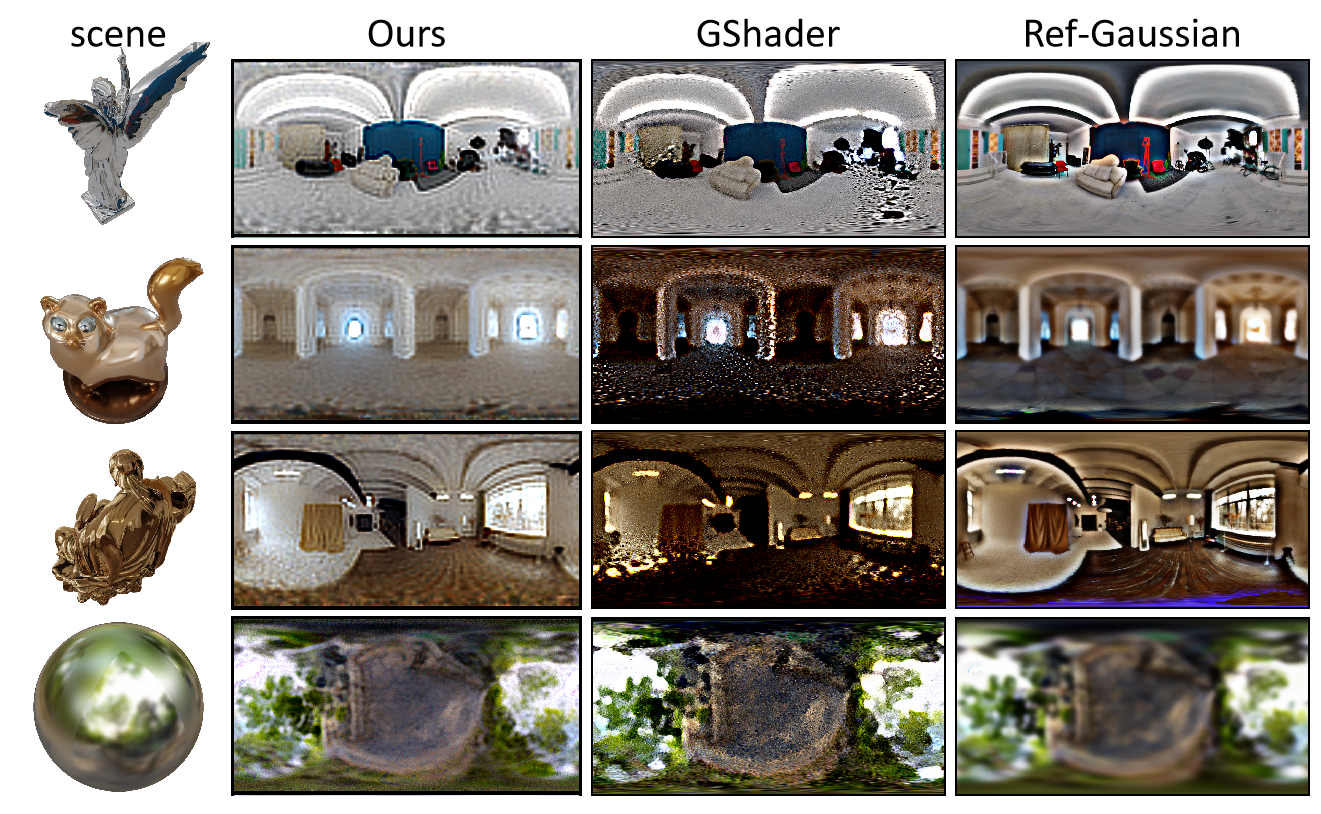
\includegraphics[width=1\linewidth]{res/envmap_compa.png}
    \captionsetup{width=0.9\linewidth}
    \caption{Qualitative comparisons of the estimated environment maps.}
    \label{fig:envmap_compa}
    \vspace{-1em}
\end{figure}
%-------------------------------------------------------------------------
\subsection{Comparison}
\textbf{Novel View Synthesis.} 
Tab.~\ref{tab:quality_compa} shows quantitative comparisons against SOTA across multiple datasets, including average metric scores per dataset. Our first-stage (Sec.~\ref{sec:method-geo}) consistently outperforms SOTA across all metrics, with notable gains on Glossy Synthetic~\cite{liu2023nero} due to geometric priors. Although second-stage results (Sec.~\ref{sec:method-ir}) exhibit a modest decrease in NVS performance, they yield significantly more accurate material decomposition, as validated by subsequent relighting experiments. 
Fig.~\ref{fig:results} illustrates the output decomposition: geometry (via normals), material properties, visibility, indirect illumination, and specular compensation. Our normals are smoother and more accurate, while material decomposition adheres better to physical constraints, effectively disentangling geometry and materials for photorealistic rendering.
Fig.~\ref{fig:envmap_compa} compares the estimated environment maps. Our method effectively disentangles illumination from scene properties. Versus Ref-Gaussian~\cite{yao2024refgaussian} and GShader~\cite{jiang2024gaussianshader}, we obtain more refined maps with sharper details, fewer artifacts, and closer to ground truth.

{
\setlength{\parindent}{0pt} 
\textbf{Geometry Reconstruction.}  
Tab.~\ref{tab:normal_compa} quantitatively validates our superior normal map quality, attributable to first-stage geometry optimization. 
Fig.~\ref{fig:normal_compa} and Fig.~\ref{fig:nvs_normal_compa} further illustrate our advantage. The qualitative comparison in Fig.~\ref{fig:normal_compa} demonstrates our method's comprehensive detail capture, such as the base of a cat, cup bottom, and horse back.
Fig.~\ref{fig:nvs_normal_compa} compares our approach to competitors on glossy objects. While competitors achieve adequate novel view synthesis, they fail to reconstruct accurate geometry or precise indirect illumination in inter-reflection regions. In contrast, our method leverages geometric priors to recover precise inter-reflection geometry and generates physically consistent indirect illumination via ray tracing, producing realistic light bounces (red boxes) absent in competitors. Our solution consistently delivers accurate normals and photorealistic indirect illumination, critical for high-quality novel view synthesis in reflective scenes.
}

\begin{figure}
    \centering
    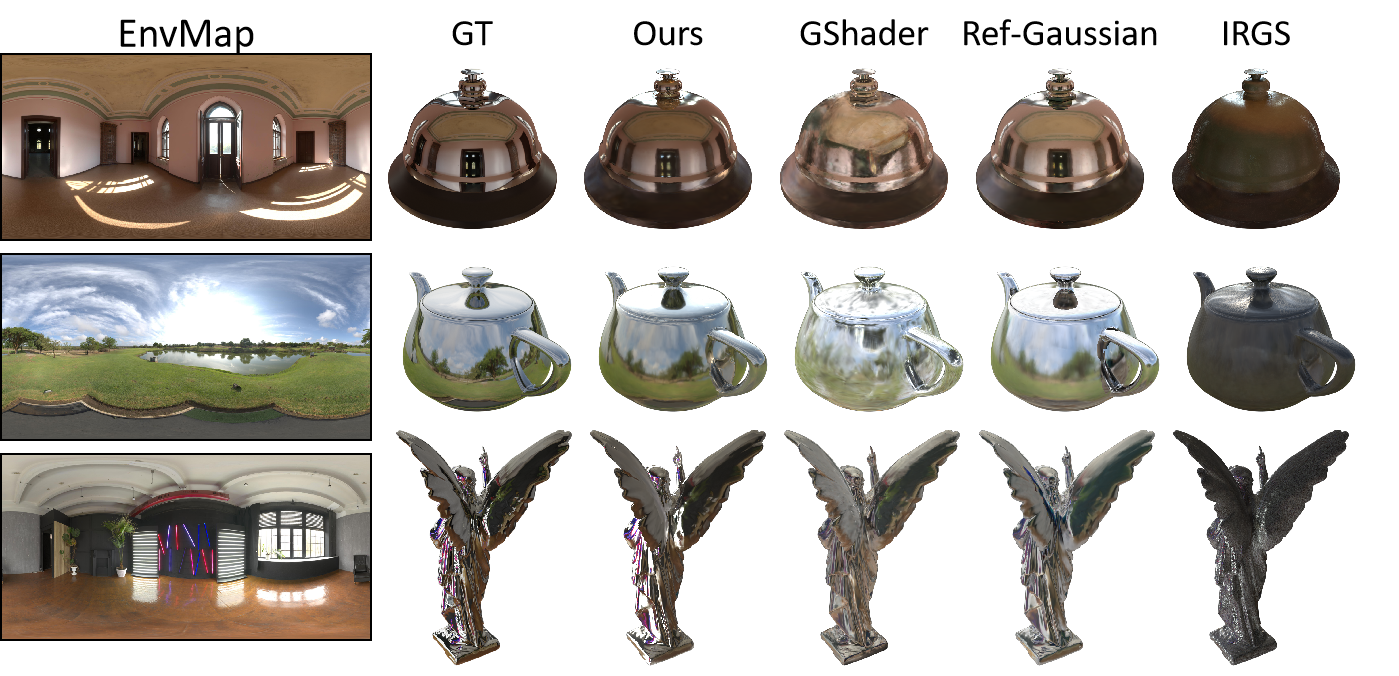
\includegraphics[width=1\linewidth]{res/relight_compa.png}
    \captionsetup{width=0.9\linewidth}
    \caption{Qualitative comparison of relighting results on the Glossy Synthetic dataset~\cite{liu2023nero}.}
    \label{fig:relight_compa}
    \vspace{-1em}
\end{figure}

\begin{figure*}[h!]
    \vspace{-1em}
    \centering
    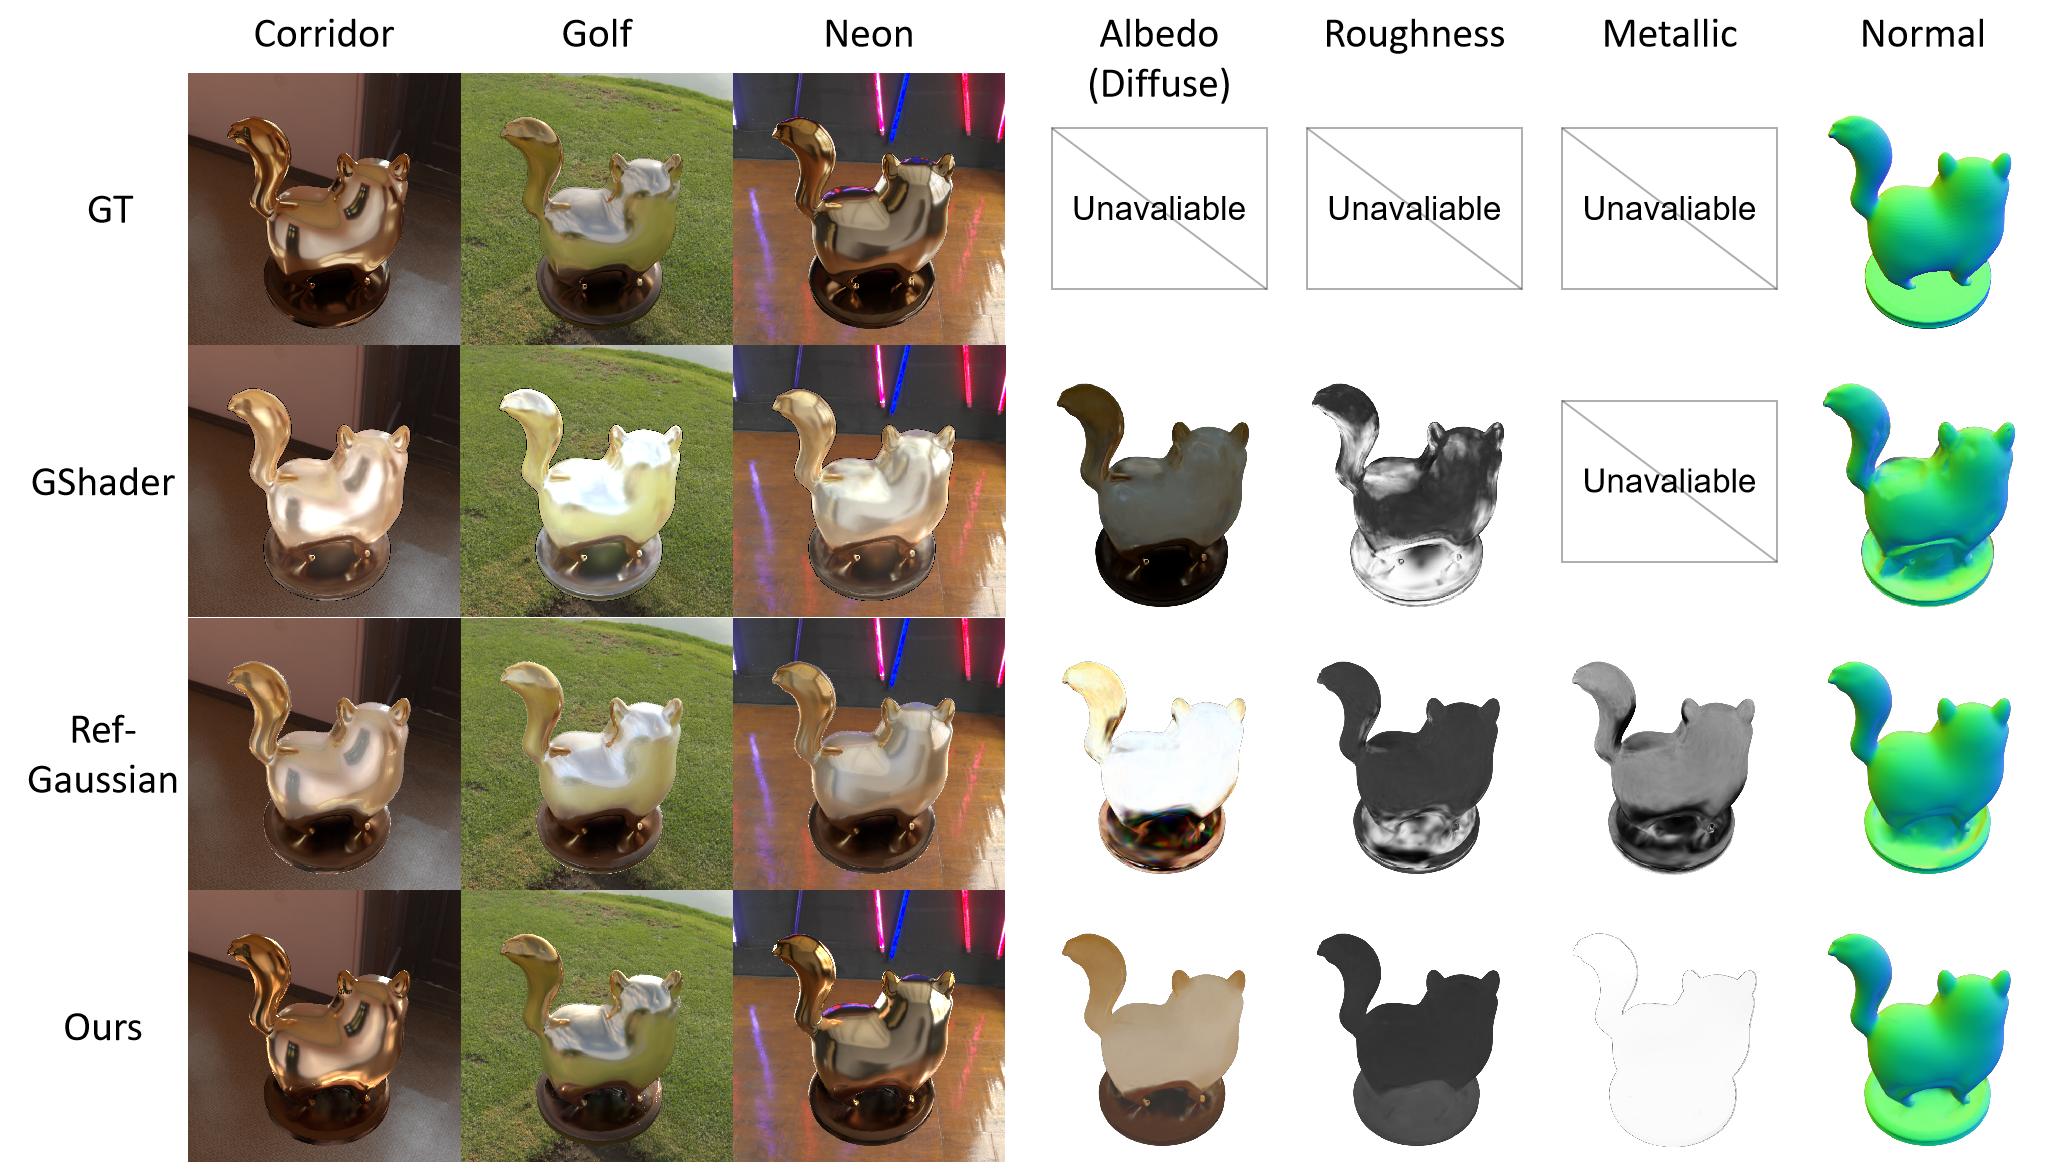
\includegraphics[width=0.84\textwidth]{res/cat_compa.png}
    \captionsetup{width=0.85\textwidth}
    \caption{Qualitative comparison of normal, material, and lighting estimation, and relighting results (using the Corridor, Golf, and Neon light maps) on the “cat” scene of the Glossy Synthetic Dataset~\cite{liu2023nero}.}
    \label{fig:cat_compa}
    \vspace{-1em}
\end{figure*}

\begin{figure}
    \centering
    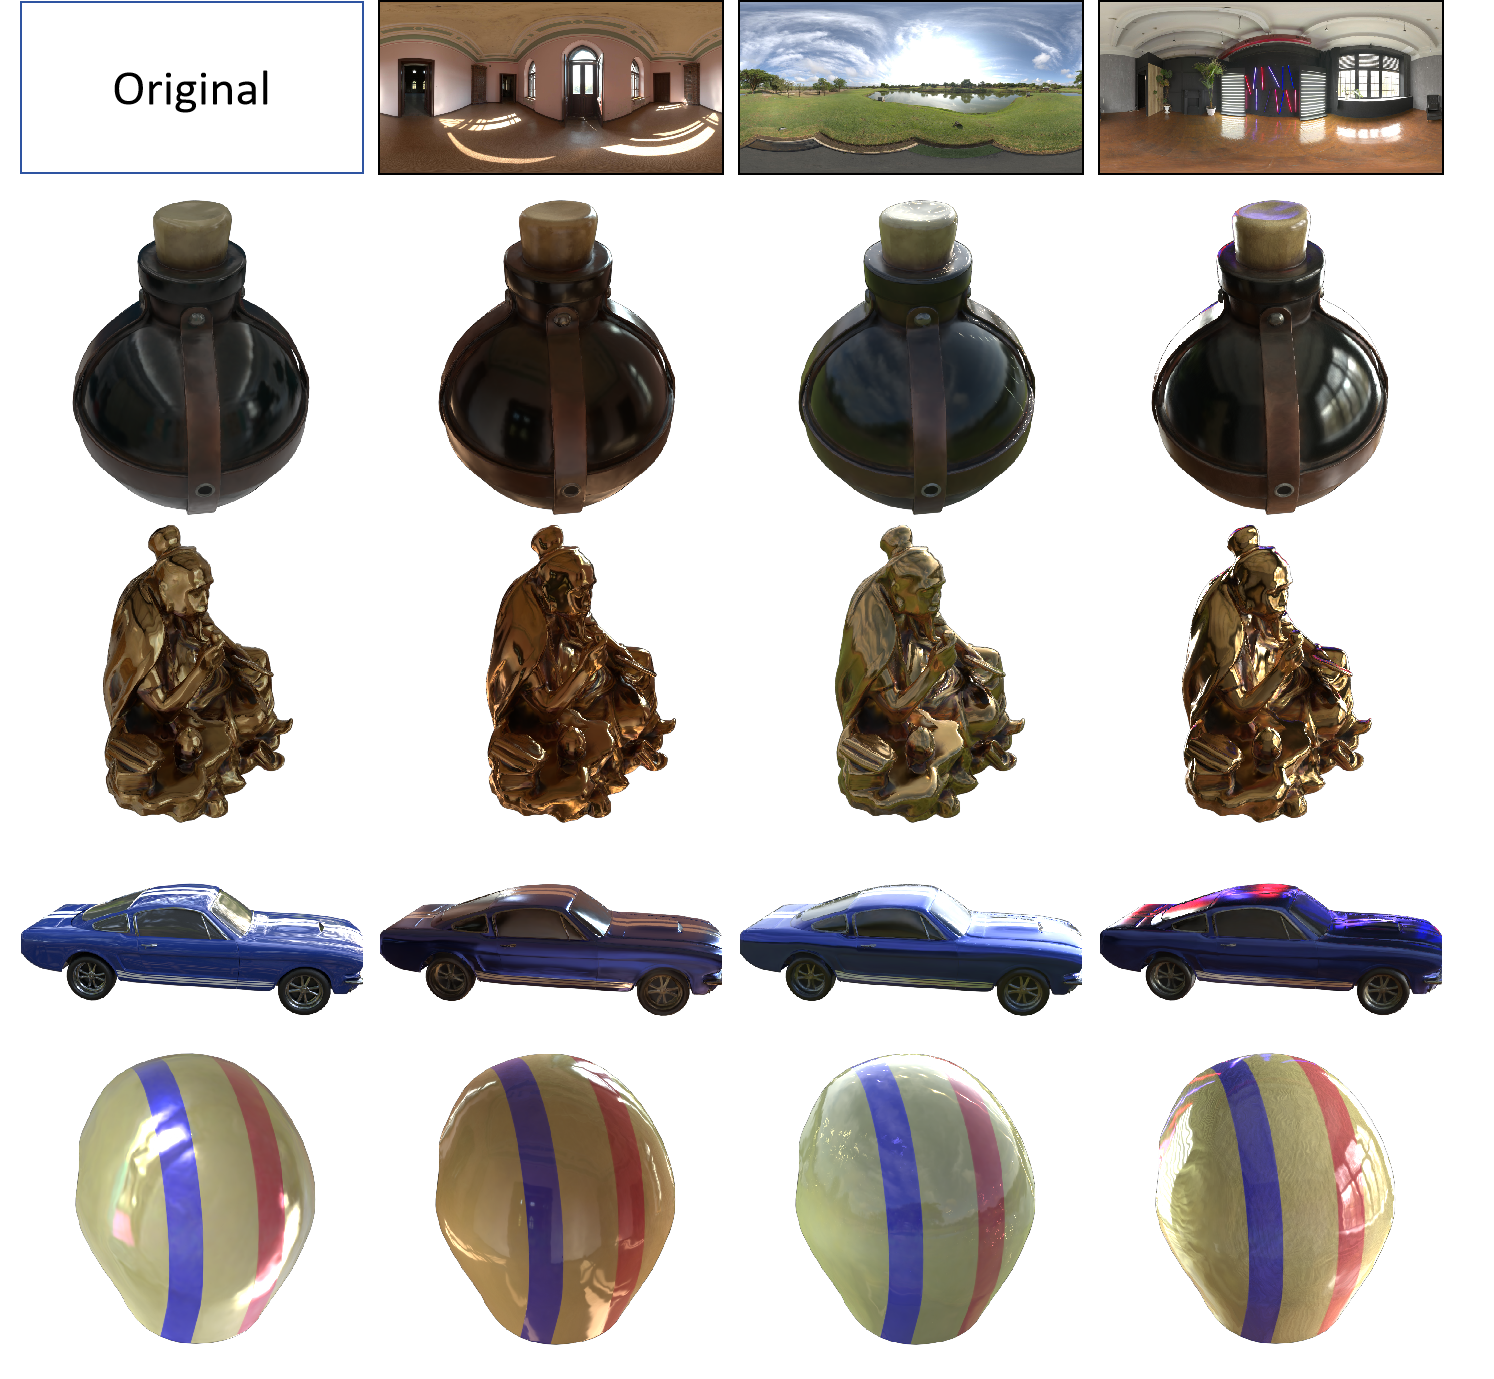
\includegraphics[width=0.9\linewidth]{res/relight_results.png}
    \captionsetup{width=0.9\linewidth}
    \caption{Relighting results on the Glossy Synthetic~\cite{liu2023nero} and Shiny Blender dataset~\cite{verbin2022refnerf}.}
    \label{fig:relight_results}
    \vspace{-1em}
\end{figure}
{
\setlength{\parindent}{0pt} % 只在当前分组内有效
\textbf{Relighting.}  
Tab.~\ref{tab:relight_psnr} shows our method achieves superior relighting quality on the Glossy Synthetic dataset~\cite{liu2023nero}, outperforming Gaussian-based approaches. 
Qualitative results in Fig.~\ref{fig:relight_compa} demonstrate our inverse rendering produces realistic specular highlights where competitors fail: GShader~\cite{jiang2024gaussianshader} exhibits geometric and material artifacts, IRGS~\cite{gu2025irgs} is limited to diffuse objects, and Ref-Gaussian's simplified rendering equation~\cite{yao2024refgaussian}  yields inaccurate material decomposition despite strong geometry. 
Fig.~\ref{fig:cat_compa} compares our "cat" reconstruction with GS-based methods~\cite{jiang2024gaussianshader, yao2024refgaussian}, showcasing high-fidelity material estimation. 
Additional relighting results for low-metallic objects (Fig.~\ref{fig:relight_results}) further validate the versatility of our method across diverse material types.
}
%-------------------------------------------------------------------------

\subsection{Ablation Study}
In Tab.~\ref{tab:ablation}, we conduct an ablation study to demonstrate the contributions of our method. First, we ablate the geometric prior supervision in the first stage and observe a minor performance drop—this is because the geometric prior supervision primarily acts on inter-reflection regions, which have limited impact on overall performance. Second, we ablate the importance sampling in the inverse rendering stage and notice a substantial performance drop, demonstrating the necessity of importance sampling for smooth object reconstruction and accurate estimation of materials and illumination. Finally, we ablate the specular compensation and once again observe a performance drop, which highlights its benefit to photorealistic reconstruction of glossy objects.


\begin{table}[]
\centering
\captionsetup{width=0.9\linewidth}
\caption{Ablation study on the Glossy Synthetic dataset~\cite{liu2023nero}.}
\label{tab:ablation}
\resizebox{\columnwidth}{!}{%
\begin{tabular}{c|ccc}
\hline
\hline
\multicolumn{1}{l|}{} & \textbf{PSNR↑} & \textbf{SSIM↑} & \textbf{LPIPS↓} \\ \hline
w/o geometry prior & 29.36 & 0.947 & 0.061 \\
w/o important sampling & 28.09 & 0.930 & 0.080 \\
w/o specular compensation & 28.58 & 0.939 & 0.067 \\
Ours & \textbf{29.38} & \textbf{0.947} & \textbf{0.061} \\ \hline \hline
\end{tabular}%
}
\vspace{-1em}
\end{table}